
\begin{frame}
\frametitle{Objekte und Merkmale}
\begin{block}{Grundbegriffe}
\begin{itemize}
\pause
\item \textit{Objekte} sind Untersuchungsgegenstände/Merkmalsträger deren Eigenschaften erhoben bzw. gemessen werden
\pause
\item Die \textit{Grundgesamtheit} bezeichnet die Menge aller Objekte
\pause
\item Oft ist eine Untersuchung aller Objekte nicht möglich, daher wird eine \textit{Stichprobe}, d.h. eine (möglichst) repräsentative Auswahl von Objekten erhoben
\pause
\item Die \textit{Stichprobenumfang} ist die Anzahl der Objekte einer Stichprobe
\pause
\item \textit{Merkmale (Variablen)} sind die (beschreibenden) Eigenschaften der Objekte
\pause
\item Eine \textit{Merkmalsausprägung} ist der konkrete Wert (aus einem Wertebereich) eines Merkmals
\end{itemize}
\end{block}
\end{frame}

%\begin{frame}
%\frametitle{Ein Beispiel}
%Studenten, die LDV besuchen:\\[0.5cm]\pause
%\begin{tabular}{l|l|r|l|c|c}
%Vorname & Name & Matrikelnummer & Studiengang & Fachsemester & Wöchentliche Lernzeit in [h]\\
%\hline
%Karl Heinz & Meier & 534521 & Logistik & 5 & 28,3\\
%Johanna & Peters & 534322 & Wirt.-Ing. & 5 & 30,4\\
%Robert & Hund & 534448 & Logistik & 5 & 33,2\\
%Thorsten & Jäger & 501203 & Logistik & 7 & 29,1\\
%Jean & Dupont & 531354 & Informatik & 5 & 25,4\\
%\multicolumn{1}{c|}{$\vdots$} & \multicolumn{1}{c|}{$\vdots$} & $\vdots$ & \multicolumn{1}{c|}{$\vdots$} & $\vdots$ & \multicolumn{1}{c}{$\vdots$}\\
%\end{tabular}
%$~$\\[0.5cm]\pause
%\begin{itemize}
%\item Jeder Student ist ein Objekt\pause
%\item Jeder Student wird durch die Merkmale Name, Vorname, Matrikelnummer, Studiengang, Fachsemester und wöchentliche Studienzeit beschrieben\pause
%\item Jedes Merkmal besitzt einen Wertebereich, etwa ist die Matrikelnummer eine natürliche Zahl und die wöchentl. Lernzeit eine positive reelle Zahl
%\end{itemize}
%\end{frame}

\begin{frame}
\frametitle{Skalenniveaus}
Verschiedene Merkmale weisen verschiedene Skalen auf:\\[0.5cm]
\pause
\begin{tabular}{l|l|l|l|l}
Skalentyp & Aussagen/Operationen & qualitativ/quantitativ & messb. Eigenschaften & Beispiel\\
\hline
Nominal & gleich, ungleich & qualitativ & Häufigkeit & Studiengänge\\[3pt]
\pause
Ordinal & gleich, ungleich,  & qualitativ & Häufigkeit, Reihenfolge & Klausurnoten\\
		& größer, kleiner 	&				& & \\[3pt]
		\pause
Intervall & gleich, ungleich & quantitativ & Häufigkeit, Reihenfolge, & IQ-Skala\\
		& größer, kleiner, & 				& Abstand & \\
		& Summe, Differenz &				&				&\\[3pt]
		\pause
Verhältnis & gleich, ungleich & quantitativ & Häufigkeit, Reihenfolge, & \\
		& größer, kleiner, & 				& Abstand, & \\
		& Summe, Differenz, &				& natürlicher Nullpunkt				& Preise\\
		& Multiplikation, Division & & &\\[3pt]
\end{tabular}
\end{frame}

\begin{frame}
\frametitle{Unterschied zwischen \textit{stetig} und \textit{diskret}}
\pause
\begin{tabular}{l|l|l}
Merkmalstyp & Anzahl der Ausprägungen & Beispiel\\
\hline
Diskret & Endlich viele & Studiengänge\\
		& abzählbar (unendlich) viele & Kontoguthaben\\[3pt]
Stetig	& Überabzählbar viele & Körpergröße
\end{tabular}
\pause
\\[0.5cm]
Erläuterung:
\begin{itemize}
\item \textit{Endlich viele} bedeutet, dass die Anzahl der Objekte endlich und zählbar ist
\pause
\item \textit{Abzählbar (unendlich) viele} bedeutet, dass die Anzahl weiterhin zählbar ist, die Anzahl der Objekte aber unendlich groß ist. Vergleiche die Menge $\mathbb{N}$ oder $\mathbb{Q}$
\pause
\item \textit{Überabzählbar viele} bedeutet, dass die Anzahl nicht mehr zählbar und unendlich ist. Vergleiche die Menge $\mathbb{R}$ oder das Intervall $[0,1]$
\end{itemize}
\end{frame}

%\begin{frame}
%\frametitle{Häufigkeiten}
%\begin{itemize}
%\item Gegeben: Beobachtungen $x_1,x_2,\ldots,x_n$ eines Merkmals $X$
%\pause
%\item $H_a$ bezeichnet die \textit{absolute Häufigkeit} einer Merkmalsausprägung $a$
%\pause
%\item Es gilt $H_a = \# \{x_i | x_i=a \}$ und $\sum_a H_a = n$
%\pause
%\item $h_a$ bezeichnet die \textit{relative Häufigkeit} der Merkmalsausprägung $a$, d.h. \[
%h_a = \frac{H_a}{n} \]
%\pause
%\item Es gilt $\sum_a h_a = 1$
%\pause
%\end{itemize}
%\pause
%Beispiel:\\
%Ein Versandhändler hat drei verschiedene Paketgrößen (S,M,L) zur Auswahl. In der letzten Stunde hat er den Verbrauch der Paketgrößen notiert:\\
%$\quad$S, S, M, L, L, L, M, S, S, S, M, M, M, M, S, M, L, S, M, S\\
%\pause
%Damit gilt $n = 20$ und
%\begin{align*}
%H_S &= 8 \quad\quad h_S = 0.4\\
%H_M &= 8 \quad\quad h_M = 0.4\\
%H_L &= 4 \quad\quad h_L = 0.2\\
%\end{align*}
%\end{frame}

\begin{frame}
\frametitle{Empirische Verteilungsfunktion}

%\item Die \textit{Summenhäufigkeit} $s$ einer Merkmalsausprägung $a$ ist definiert durch \[
%s_a = \frac{\#\{x_i| x_i \leq a\}}{n}
%\]
%\pause
\begin{block}{Definition}
Die \textit{empirische Verteilungsfunktion} $F_n$ ist definiert durch\[
F_n(x) = \frac{\#\{x_i| x_i \leq x\}}{n}
\]
\end{block}
\pause
\begin{center}
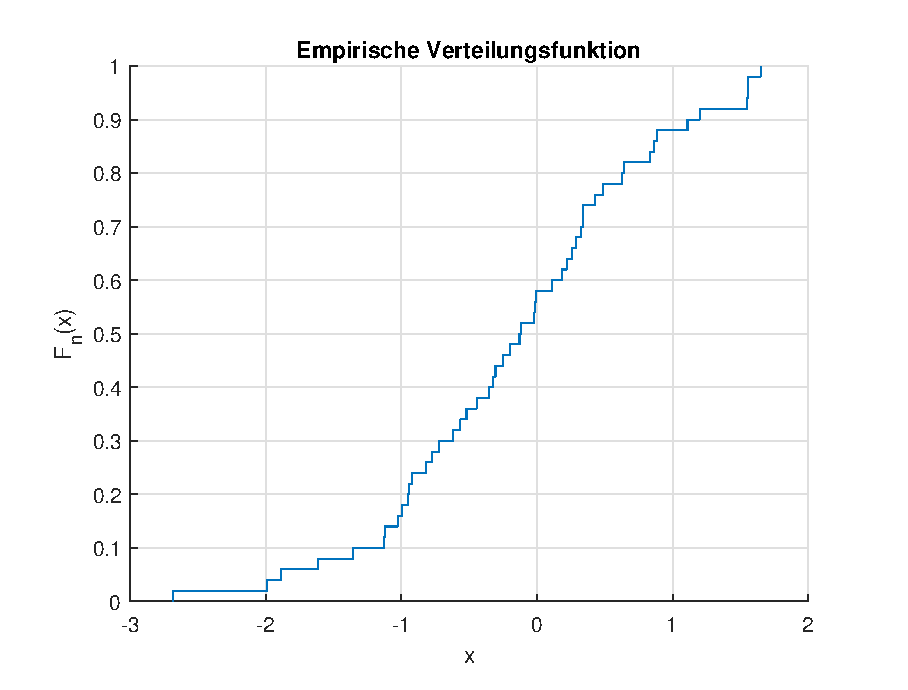
\includegraphics[scale=0.4]{images/empirische_verteilungsfunktion_bsp.eps} 
\end{center}
\end{frame}

\begin{frame}
\frametitle{Lagemaße}
\begin{itemize}
\item Lässt sich eine Stichprobe $x_1,x_2,\ldots,x_n$ sortieren, dann ist $x_{(1)},x_{(2)},\ldots,x_{(n)}$ die $sortierte$ Stichprobe mit $x_{(1)} \leq x_{(2)} \leq \ldots \leq x_{(n)}$
\pause
\item $x_{(1)} = \min\limits_{i=1,\ldots,n} x_i$   und $x_{(n)} = \max\limits_{i=1,\ldots,n} x_i$
\pause
\item $\argmax$ ist das argumentative Maximum einer Menge bzw. Funktion, d.h. der Wert bzw. die Werte an denen das Maximum angenommen wird
\end{itemize}
\pause
\begin{block}{Def.: Lagemaße}
\begin{itemize}
\item Modalwert: $\bar{x}_M := \argmax\limits_a \{H_a| a \text{ ist Merkmalsausprägung} \} $
\pause
\item arithmetisches Mittel: $\bar{x} := \frac{1}{n}\sum\limits_{i=1}^n x_i$
\pause
\item Median: $\bar{x}_{med} = \begin{cases} x_{\left(\frac{n+1}{2}\right)} &\text{ , falls } n \text{ ungerade}\\  \frac{1}{2}\left( x_{\left(\frac{n}{2}\right)} + x_{\left(\frac{n}{2}+1\right)}\right) &\text{ , falls } n \text{ gerade}\end{cases}$
\pause
\item $\alpha$-Quantil:  ${x}_\alpha = \begin{cases} x_{\left( \lfloor n\cdot\alpha+1\rfloor\right)} &\text{ , falls } n\cdot\alpha \text{ nicht ganzzahlig}\\  \frac{1}{2}\left( x_{(n \cdot \alpha)} + x_{(n\cdot \alpha +1)}\right) &\text{ , falls } n \cdot \alpha \text{ ganzzahlig}\end{cases}$ $\quad$für $\alpha \in (0,1)$
\end{itemize}
\end{block}
\end{frame}

%\begin{frame}
%\frametitle{Streuungsmaße}
%\begin{block}{Def.: Streuungsmaße}
%\begin{itemize}
%\item Empirische Varianz: $s_x^2 := \frac{1}{n}\sum_{i=1}^n (x_i-\bar{x})^2$
%\pause
%\item Empirische Standardabweichung: $s_x := \sqrt{\frac{1}{n}\sum_{i=1}^n (x_i-\bar{x})^2} = \sqrt{s_x^2}$
%\pause
%\item Mittlere absolute Medianabweichung: $\text{MD} := \frac{1}{n}\sum\limits_{i=1}^n \vert x_i - \bar{x}_{med} \vert$
%\pause
%\item Interquartilsabstand: $\text{IQA}= x_{0.75}-x_{0.25}$
%\pause
%\item Spannweite: $R=x_{(n)}-x_{(1)}$
%\end{itemize}
%\end{block}
%\end{frame}

\begin{frame}
\frametitle{Korrelationskoeffizient}
Für zwei Merkmale $X$ und $Y$ seien $(x_1,y_1),\ldots,(x_n,y_n)$ Paare von Merkmalsausprägungen.
\begin{block}{Def.: Stichprobenkovarianz und Korrelationskoeffizient}
\begin{itemize}
\pause
\item Die Stichprobenkovarianz ist definiert als
\[
s_{xy} = \frac{1}{n}\sum\limits_{i=1}^n (x_i-\bar{x})\cdot(y_i-\bar{y})
\]
\pause
\item Der Korrelationskoeffizient ist definiert als
\[
r_{xy} = \frac{\sum\limits_{i=1}^n (x_i-\bar{x})\cdot(y_i-\bar{y})}{\sqrt{\sum\limits_{i=1}^n (x_i-\bar{x})^2}\cdot \sqrt{\sum\limits_{i=1}^n (y_i-\bar{y})^2}} = \frac{s_{xy}}{s_x\cdot s_y}
\]
\end{itemize}
\end{block}
\end{frame}

\begin{frame}
\frametitle{Korrelation vs. Kausalität}
\begin{itemize}[<+->]
\item Korrelation: Zwei Merkmale sind korreliert, wenn sie einen von Null signifikant verschiedenen Korrelationskoeffizienten aufweisen! Das heißt auf Datenebene besteht ein Zusammenhang
\item Kausalität: Zwei Merkmale sind kausal abhängig, wenn zwischen ihnen ein Ursache-Wirkung Zusammenhang besteht
\end{itemize}
\pause
\begin{block}{Achtung!}
\textbf{Korrelation $\neq$ Kausalität}\\
Mittels statistischer Methoden kann nur eine Korrelation, nie eine Kausalität, nachgewiesen werden! (Das heißt aber noch lange nicht, dass keine Kausalität vorliegt.)
\end{block}
\end{frame}

\begin{frame}
\begin{figure}[hbtp]
\centering
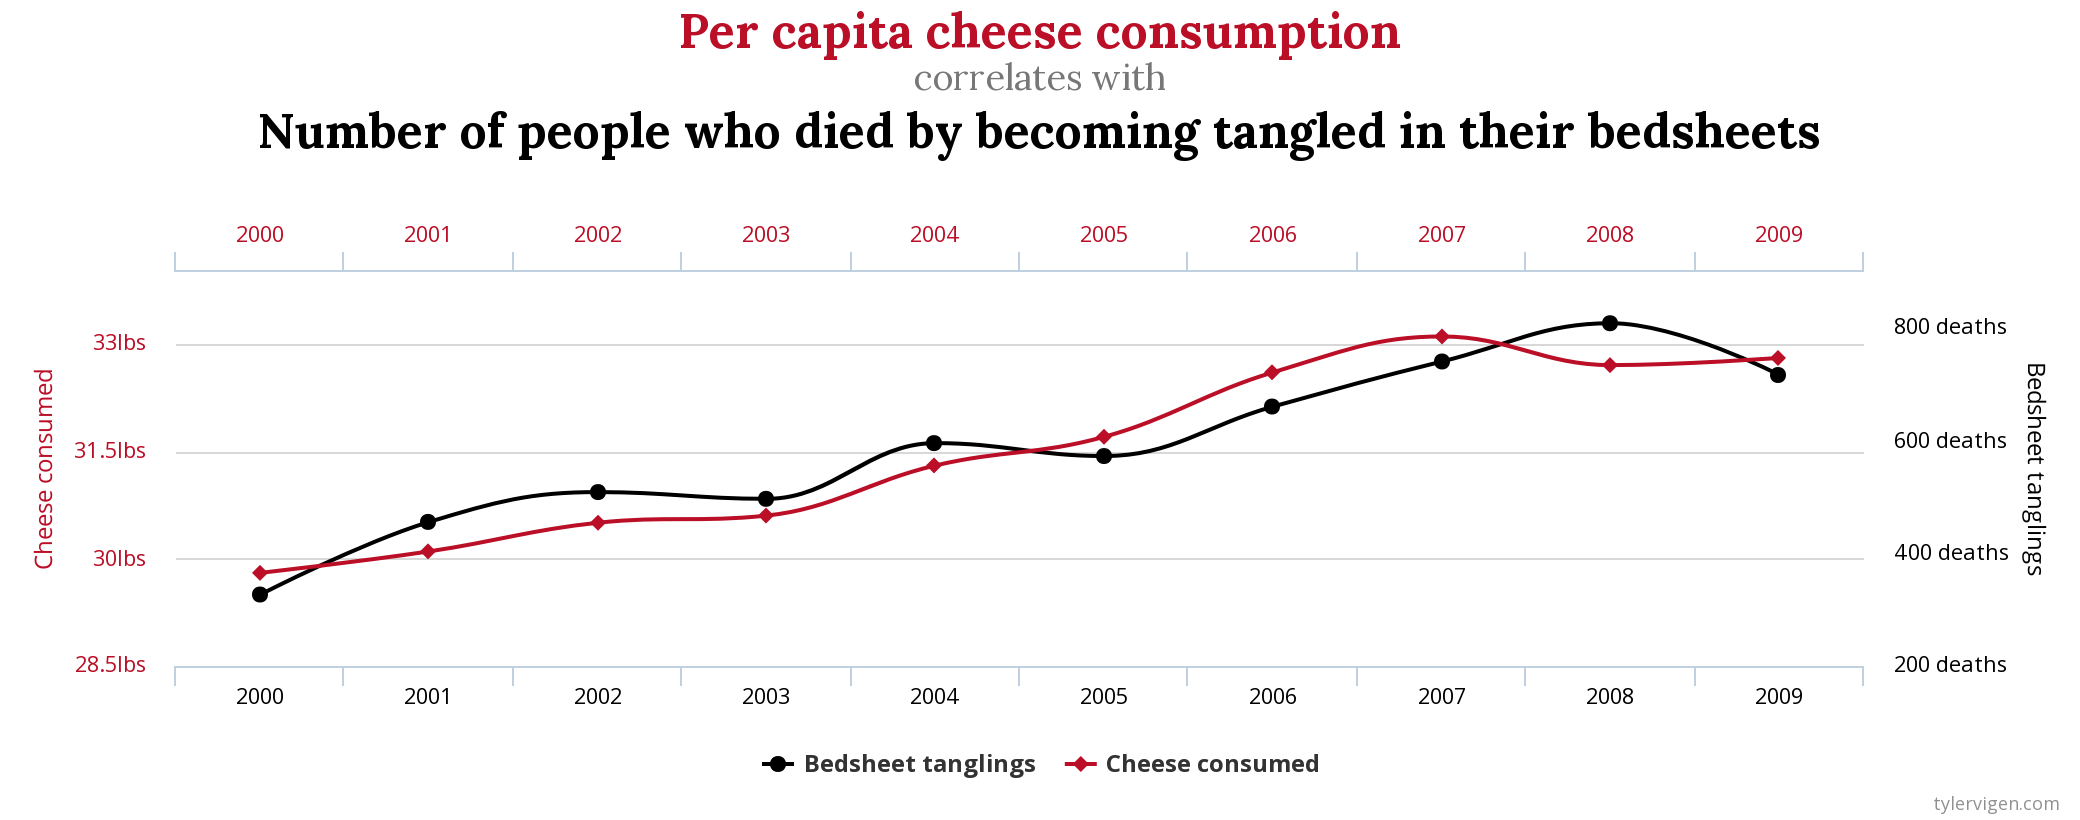
\includegraphics[scale=0.2]{images/chart-korrelation.png}
\caption{Beispiel für eine Korrelation, bei der kein kausaler Zusammenhang besteht ($r_{xy} = 0.947091$). Quelle: Entnommen von http://www.tylervigen.com/spurious-correlations}
\end{figure}
\end{frame}

%\begin{frame}
%\frametitle{Mengenoperationen}
%Seien $A$ und $B$ Teilmengen von $\Omega$, d.h. $A \subseteq \Omega$ und $B \subseteq \Omega$. Dann ist
%\begin{itemize}
%\item $A\cup B$ die \textit{Vereinigung} der Mengen $A$ und $B$, d.h. $A\cup B = \lbrace x \in \Omega~  | x\in A \vee x\in B\rbrace$\footnote{Das \glqq oder \grqq{} ($\vee$) ist wie üblich nicht-exklusiv gemeint, d.h. $x$ kann sowohl Element von $A$, als auch von $B$ sein.}
%\pause
%\item $A \cap B$ der \textit{Schnitt} der Mengen $A$ und $B$, d.h. $A\cap B = \lbrace x \in \Omega~ | x\in A \wedge x\in B\rbrace$
%\pause
%\item $A \setminus B$ die \textit{Differenz} von $A$ und $B$ (\glqq $A$ ohne $B$\grqq), d.h. $A\setminus B = \lbrace x \in \Omega~ | x\in A \wedge x\notin B\rbrace$
%\pause
%\item $A^C$ das Komplement von $A$, d.h. $A^C = \lbrace x \in \Omega~ | x \notin A \rbrace$
%\pause
%\item $A \times B$ das \textit{kartesische Produkt} von $A$ und $B$, d.h. $A\times B = \lbrace (x,y)\in\Omega ~ | x\in A \wedge y\in B \rbrace$
%\end{itemize}
%\end{frame}

\begin{frame}
\frametitle{Wahrscheinlichkeitstheorie}
\begin{tabular}{l|c|l|l}
Begriff & Symbol & Erläuterung & Beispiel\\
\hline
\pause
Zufallsexperiment & & Prozess zur Erhebung von Daten  &Werfen eines \\
				& &mit nicht vorhersagbarem Ausgang	&			6-seitigen Würfels\\[3pt]
\pause
Ergebnis &$\omega$& Elementarer Ausgang eines  & 3\\
	&  & Zufallsexperiments & \\[3pt]
\pause
Grundraum &$\Omega$& Menge aller möglicher Ergebnisse & $\{1,2,3,4,5,6\}$\\[3pt]
\pause
Ereignis&z.B. $A$& Menge von Ergebnissen, also eine  & $A = \text{\glqq Das Ergebnis ist gerade\grqq}$ \\	
		& & Teilmenge des Grundraums & bzw. $A=\{2,4,6\}$\\[3pt]
\pause
Wahrscheinlichkeits- & $P$ & Gibt die Wahrscheinlichkeit  & $P(A) = \frac{1}{2}$\\
maß & & von Ereignissen an\footnote{$P$ ist eine Funktion von einem geeigneten Mengensystem (einer $\sigma$-Algebra) in das Intervall $[0,1]$.} & \\
\end{tabular}
\end{frame}

%\begin{frame}
%\frametitle{Wichtige Rechenregeln}
%Seien $A$ und $B$ zwei Ereignisse, dann gelten die folgenden Regeln
%\begin{itemize}
%\item $A \cap B = \varnothing \Rightarrow P(A \cup B ) = P(A) + P(B)$
%\pause
%\item $A \subseteq B \Rightarrow P(B\setminus A) = P(B)-P(A)$
%\pause
%\item $P(A \cup B) = P(A)+P(B)-P(A \cap B)$
%\pause
%\item $P(A^c) = 1-P(A)$
%\pause
%\item $A$ und $B$ heißen \textit{stochastisch unabhängig} genau dann, wenn $P(A\cap B) = P(A) \cdot P(B)$ gilt\footnote{Gilt für zwei Ereignisse $P(A\cap B) \neq P(A) \cdot P(B)$ , so wird dies nicht \glqq stochastisch abhängig\grqq{} genannt, sondern \glqq nicht stochastisch unabhängig\grqq{}.}
%\end{itemize}
%\end{frame}

%\begin{frame}
%\frametitle{Der Satz von Bayes I}
%\pause
%\begin{block}{Def.: bedingte Wahrscheinlichkeit}
%Die \textit{bedingte Wahrscheinlichkeit}, dass $A$ unter der Bedingung $B$ eintritt, ist definiert als
%\begin{equation*}
%P(A|B) := \frac{P(A \cap B)}{P(B)},
%\end{equation*}
%für $P(B) > 0$.\\
%$P(A|B)$ ist also die Wahrscheinlichkeit, dass $A$ eintritt, wenn $B$ bereits eingetreten ist.
%\end{block}
%\pause
%Beispiel: Unter einem Würfelbecher liegt verdeckt ein Würfel. Es sei bekannt, dass die obenliegende Augenzahl ungerade sei, d.h. $B=\{1,3,5\}$. Wie groß ist die Wahrscheinlichkeit, dass die Augenzahl gleich $3$ ist, sprich $A=\{3\}$?\\
%\pause
%\[
%P(A|B) = \frac{P(A \cap B)}{P(B)} = \frac{P(\{1,3,5\} \cap \{3\})}{P(\{1,3,5\})} = \frac{P(\{3\})}{P(\{1,3,5\})} = \frac{\frac{1}{6}}{\frac{1}{2}} = \frac{1}{3}
%\]
%Umgekehrt gilt: $P(B|A) = 1$
%\end{frame}
%
%\begin{frame}
%\frametitle{Der Satz von Bayes II}
%\begin{block}{Der Satz von Bayes}
%\begin{itemize}[<+->]
%\item[(1)] Seien $A$ und $B$ zwei Ereignisse mit $P(A)>0$ und $P(B)>0$. Dann gilt
%\[
%P(A|B) = \frac{P(B|A)\cdot P(A)}{P(B)}.
%\]
%\item[(2)] Seien $B_1,\ldots,B_m$ und $A$ Ereignisse mit $P(B_i)>0$ für $i=1,\ldots,m$, $P(A)>0$, $B_i \cap B_j = \varnothing$ für $i\neq j$ und $\bigcup\limits_{i=1}^m B_i = \Omega$. Dann gilt
%\[
%P(B_k|A) = \frac{P(A|B_k)\cdot P(B_k)}{\sum\limits_{i=1}^m P(A|B_i)\cdot P(B_i)}
%\]
%\end{itemize}
%\end{block}
%\end{frame}

%\begin{frame}
%\frametitle{Beispiel zum Satz von Bayes}
%\begin{itemize}
%\item Szenario: Ein Bauteil wird auf seine Funktionsfähigkeit untersucht. Ein Leuchtdiode an dem Prüfgerät zeigt an, ob das Bauteil den Test bestanden hat.
%\pause
%\item Bekannt: $1\%$ aller Bauteile sind defekt,\\
%\pause
%$\quad\quad\quad\quad$Ist ein Bauteil defekt, so meldet das Prüfgerät dies in $95\%$ der Fälle,\\
%\pause
%$\quad\quad\quad\quad$In $0.5\%$ der Fälle, in denen ein Bauteil nicht defekt ist, wird dennoch ein Defekt gemeldet
%\pause
%\item Frage 1: Wie groß ist die Wahrscheinlichkeit, dass ein Bauteil bei dem das Prüfgerät einen Defekt meldet, auch wirklich defekt ist?
%\pause
%\item Frage 2: Wie groß ist die Wahrscheinlichkeit, dass ein Bauteil, das als nicht defekt eingestuft wird, auch wirklich nicht defekt ist?
%\pause
%\item Frage 3: Sind die Ereignisse \glqq Bauteil ist defekt\grqq{} und \glqq Prüfgerät meldet einen Defekt\grqq{} stochastisch unabhängig?
%\end{itemize}
%\end{frame}

\begin{frame}
\frametitle{Lösung}
\begin{itemize}[<+->]
\item Definiere 
\begin{align*}
A &= \lbrace \text{Bauteil ist defekt}\rbrace \\
B &= \lbrace \text{Prüfgerät meldet einen Defekt}\rbrace
\end{align*}
\item Dann gilt nach Aufgabenstellung
\[ P(A) = 0.01, \quad P(B|A) = 0.95, \quad P(B|A^C) = 0.005\]
\end{itemize}
\end{frame}

%\begin{frame}
%\frametitle{Lösung Frage 1}
%Frage 1: Wie groß ist die Wahrscheinlichkeit, dass ein Bauteil bei dem das Prüfgerät einen Defekt anzeigt auch wirklich defekt ist?\\
%Gesucht ist $P(A|B)$. Es gilt \pause
%\begin{align*}
%P(A|B) 	&= \frac{P(B|A)\cdot P(A)}{P(B)} \\
%		&= \frac{P(B|A)\cdot P(A)}{P(B|A)\cdot P(A) + P(B|A^C) \cdot P(A^C)}\\
%		&= \frac{0.95 \cdot 0.01}{0.95 \cdot 0.01 + 0.005 \cdot (1-0.01)}\\
%		&= \frac{190}{289}\\
%		&\approx 65.74 \%
%\end{align*}
%\end{frame}
%\begin{frame}
%\frametitle{Lösung Frage 2}
%Wie groß ist die Wahrscheinlichkeit, dass ein Bauteil, das als nicht defekt eingestuft wird, auch wirklich nicht defekt ist?
%Gesucht ist $P(A^C|B^C)$. Es gilt \pause
%
%\begin{align*}
%P(A^C|B^C) 	&= \frac{P(B^C|A^C)\cdot P(A^C)}{P(B^C)} \\
%		&= \frac{P(B^C|A^C)\cdot P(A^C)}{P(B^C|A^C)\cdot P(A^C) + P(B^C|A) \cdot P(A)}\\
%		&= \frac{(1-P(B|A^C))\cdot (1-P(A))}{(1-P(B|A^C))\cdot (1-P(A)) + (1-P(B|A)) \cdot P(A)}\\
%		&= \frac{(1-0.005) \cdot (1-0.01)}{(1-0.005) \cdot (1-0.01) + (1-0.95) \cdot 0.01}\\
%		&= \frac{19701}{19711}\\
%		&\approx 99.99 \%
%\end{align*}
%\end{frame}
%\begin{frame}
%\frametitle{Lösung Frage 3}
%Sind die Ereignisse \glqq Bauteil ist defekt\grqq und \glqq{} Prüfgerät erkennt einen Defekt\grqq{} stochastisch unabhängig?
%Es gilt \pause
%\begin{align*}
%P(A) 	&= 0.01 \\
%P(B) 	&= P(B|A)\cdot P(A) + P(B|A^C) \cdot P(A^C)\\
%		&= 0.95 \cdot 0.01 + 0.005 \cdot (1-0.01)\\
%		&= 0.01445
%\end{align*}
%und daher 
%\[
%P(A)\cdot P(B) = 0.0001445 \neq 0.0095 = P(A|B)\cdot P(B) = P(A\cap B) 
%\]
%und somit sind $A$ und $B$ nicht stochastisch unabhängig.\footnote{Äquivalent kann überprüft werden ob $P(A|B) \neq P(A)$ gilt, denn zwei Ereignisse sind gdw. stochastisch unabhängig wenn $P(A|B) = P(A)$ gilt.}
%\end{frame}

%\begin{frame}
%\frametitle{Zufallsvariablen}
%\begin{itemize}[<+->]
%\item Eine \textit{Zufallsvariable}, auch Zufallsgröße genannt, ist eine Vorschrift, die jedem Ergebnis $\omega \in \Omega$  eines Zufallsexperimentes einen Wert zuordnet. 
%\item Zufallsvariablen werden üblicherweise mit lateinischen Großbuchstaben, wie $X,Y,\ldots$, bezeichnet
%\item Der zugeordnete Wert $X(\omega)$ wird auch Realisierung genannt
%\item Die Verteilungsfunktion einer Zufallsvariablen $X$ ist definiert\footnote{$\lbrace X \leq x \rbrace$ ist eine abkürzende Schreibweise für $\lbrace \omega\in\Omega \vert X(\omega) \leq x \rbrace$} als \[F_X(x) := P(X\leq x)\]
%\item Die gemeinsame Verteilungsfunktion zweier Zufallsvariablen $X$ und $Y$ ist definiert\footnote{Das Komma zwischen die beiden Mengen $\lbrace X\leq x\rbrace$ und $\lbrace Y \leq y \rbrace$ ist eine Kurzschreibweise für den Schnitt der beiden Mengen} als \[F_{X,Y}(x,y) := P(X\leq x, Y\leq y)\] 
%\item Für eine diskrete Zufallsvariable ist $f(x) := P(X=x)$ die sogenannte \textit{Zähldichte}
%\item Für eine stetige Zufallsvariable ist $f(x) := F_X'(x)$ (also die Ableitung der Verteilungsfunktin) die sogenannte \textit{Dichte}
%\end{itemize}
%\end{frame}
%\begin{frame}
%\frametitle{Dichten und Verteilungsfunktionen}
%Eine Dichte $f$ besitzt die folgenden definierenden Eigenschaften:
%\begin{itemize}[<+->]
%\item $f$ ist nicht-negativ, d.h. $f \geq 0$
%\item $f$ ist normiert und für stetige Verteilungen integrierbar, d.h $\sum_x f(x) = 1$ für diskrete Verteilungen und $\int f(x) dx = 1$ für stetige Verteilungen
%\item Wichtig: Eine Dichte ist eindeutig für eine Verteilung
%\end{itemize}
%Eine Verteilungsfunktion $F$ besitzt die folgenden Eigenschaften:
%\begin{itemize}[<+->]
%\item $F$ ist monoton steigend, d.h. $F(x) \leq F(y)$ für $x\leq y$
%\item $F$ ist rechtsseitig stetig
%\item Es gilt $\lim_{x\rightarrow \infty} F(x) = 1$ und $\lim_{x\rightarrow -\infty} F(x) = 0$
%\end{itemize}
%Die gemeinsame Verteilung zweier Zufallsvariablen $X$ und $Y$ ist definiert als
%\[ F_{(X,Y)}(x,y) := P(X\leq x, Y\leq y) \]
%\end{frame}

\begin{frame}
\frametitle{Erwartungswert, Varianz und Kovarianz für diskrete Zufallsvariablen}
\begin{block}{Erwartungswert, Varianz und Kovarianz}
Für zwei diskrete Zufallsvariablen $X$ und $Y$ ist
\begin{itemize}[<+->]
\item der Erwartungswert definiert als
\[ \mathbb{E}(X) := \sum_x x\cdot f(x),
\]
\item die Varianz definiert als \[
\text{Var}(X) := \mathbb{E}\left(\left(X-\mathbb{E}(X)\right)^2\right) = \sum_x \left( x-\mathbb{E}(X)\right)^2\cdot f(x)
\]
%\item die Kovarianz definiert als
%\begin{align*} 
%\text{cov}(X,Y) &:= \mathbb{E}\left( (X-\mathbb{E}(X))\cdot(Y-\mathbb{E}(Y))\right) \\
%&= \sum_{x}\sum_y P(X=x,Y=y) (x-\mathbb{E}(X)\cdot(y-\mathbb{E}(Y) 
%\end{align*}
\end{itemize}
\end{block}
\end{frame}

\begin{frame}
\frametitle{Erwartungswert, Varianz und Kovarianz für stetige Zufallsvariablen}
\begin{block}{Erwartungswert und Varianz}
Für zwei stetige Zufallsvariable ist
\begin{itemize}[<+->]
\item der Erwartungswert definiert als
\[ \mathbb{E}(X) := \int x\cdot f(x) dx,
\]
\item die Varianz definiert als \[
\text{Var}(X) := \mathbb{E}\left(\left(X-\mathbb{E}(X)\right)^2\right) = \int \left( x-\mathbb{E}(X)\right)^2\cdot f(x) dx
\]
\end{itemize}
\end{block}
\end{frame}

%\begin{frame}
%\frametitle{Rechenregeln für den Erwartungswert und die Varianz}
%Für den Erwartungswert und die Varianz zweier Zufallsvariablen $X,Y$ gelten die folgenden sehr hilfreichen Rechenregeln:
%\begin{itemize}[<+->]
%\item Transformationssatz:\[
%\mathbb{E}(g(X)) = \begin{cases} \sum_x g(x)\cdot f(x) & \text{ , falls $X$ diskret}\\ \int g(x)\cdot f(x) dx & \text{ , falls $X$ stetig} \end{cases}
%\]
%\item Linearität:
%\begin{align*}
%\mathbb{E}(a\cdot X -b) &= a\cdot\mathbb{E}(X) -b \\
%\mathbb{E}(X+Y) &= \mathbb{E}(X) + \mathbb{E}(Y)
%\end{align*}
%\item Verschiebungssatz: 
%\[
%\text{Var}(X) = \mathbb{E}(X^2) - \left(\mathbb{E}(X)\right)^2
%\]
%\item Lineare Transformation der Varianz:
%\begin{align*} 
%\text{Var}(a\cdot X -b) &= a^2\cdot\text{Var}(X) \\
%%\text{Var}(X+Y) &= \text{Var}(X) + \text{Var}(Y) - \text{cov}(X,Y)
%\end{align*}
%\end{itemize}
%\end{frame}

%\begin{frame}
%\frametitle{Die Gleichverteilung}
%\begin{block}{Gleichverteilte Zufallsvariable}
%\begin{itemize}[<+->]
%\item Eine diskrete Zufallsvariable $X$ heißt \textit{gleichverteilt} auf der Menge $T:=\lbrace x_1,\ldots,x_n\rbrace$, wenn jede ihrer Realisierungen $x_i$ gleichwahrscheinlich ist, das heißt
%\[ f_X(x_i) = \frac{1}{n} \quad\text{ für } i=1,\ldots,n.\] Kurz wird dies auch notiert als  $X\sim \mathcal{U}(T) $. Die Menge $T$ heißt auch Träger.
%\item Eine stetige Zufallsvariable $X$ heißt \textit{gleichverteilt} auf dem Intervall $[a,b]$, wenn für ihre Dichte gilt
%\[ f_X(x) = \begin{cases} \frac{1}{b-a} & \text{ , falls } x\in [a,b] \\ 0 & \text{ , sonst } \end{cases}. \] Dies wird kurz notiert als $X\sim \mathcal{U}([a,b])$.
%\end{itemize}
%\end{block}
%\end{frame}

\begin{frame}
\frametitle{Diskrete Gleichverteilung}
\begin{figure}[hbtp]
\centering
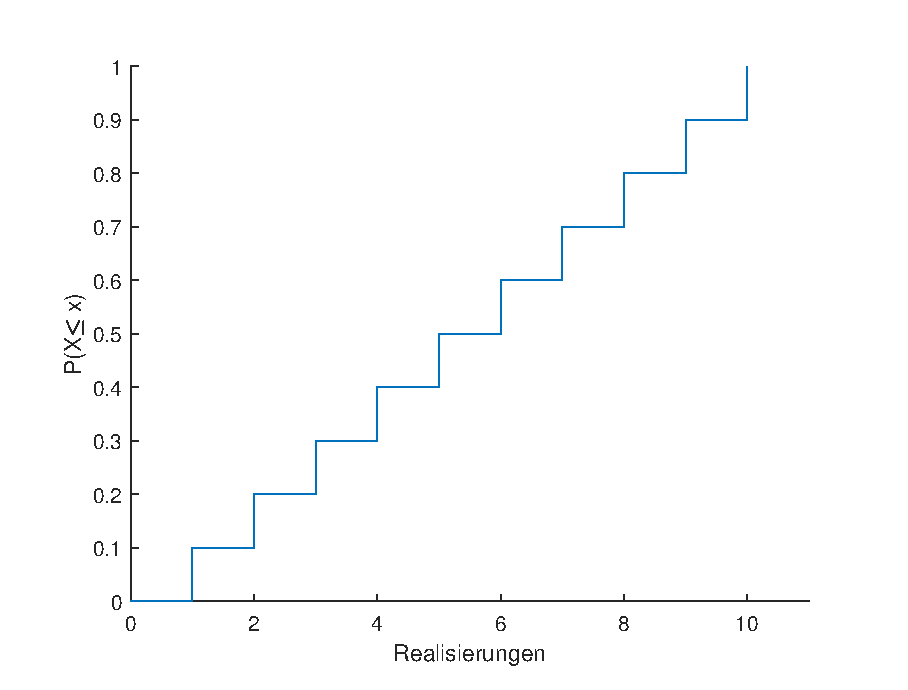
\includegraphics[scale = 0.5]{images/plot_discrete_uniform.eps}
\caption{Verteilungsfunktion einer auf {1,2,...10} gleichverteilten Zufallsvariablen}
\end{figure}
\end{frame}

\begin{frame}
\frametitle{Stetige Gleichverteilung}
\begin{figure}[hbtp]
\centering
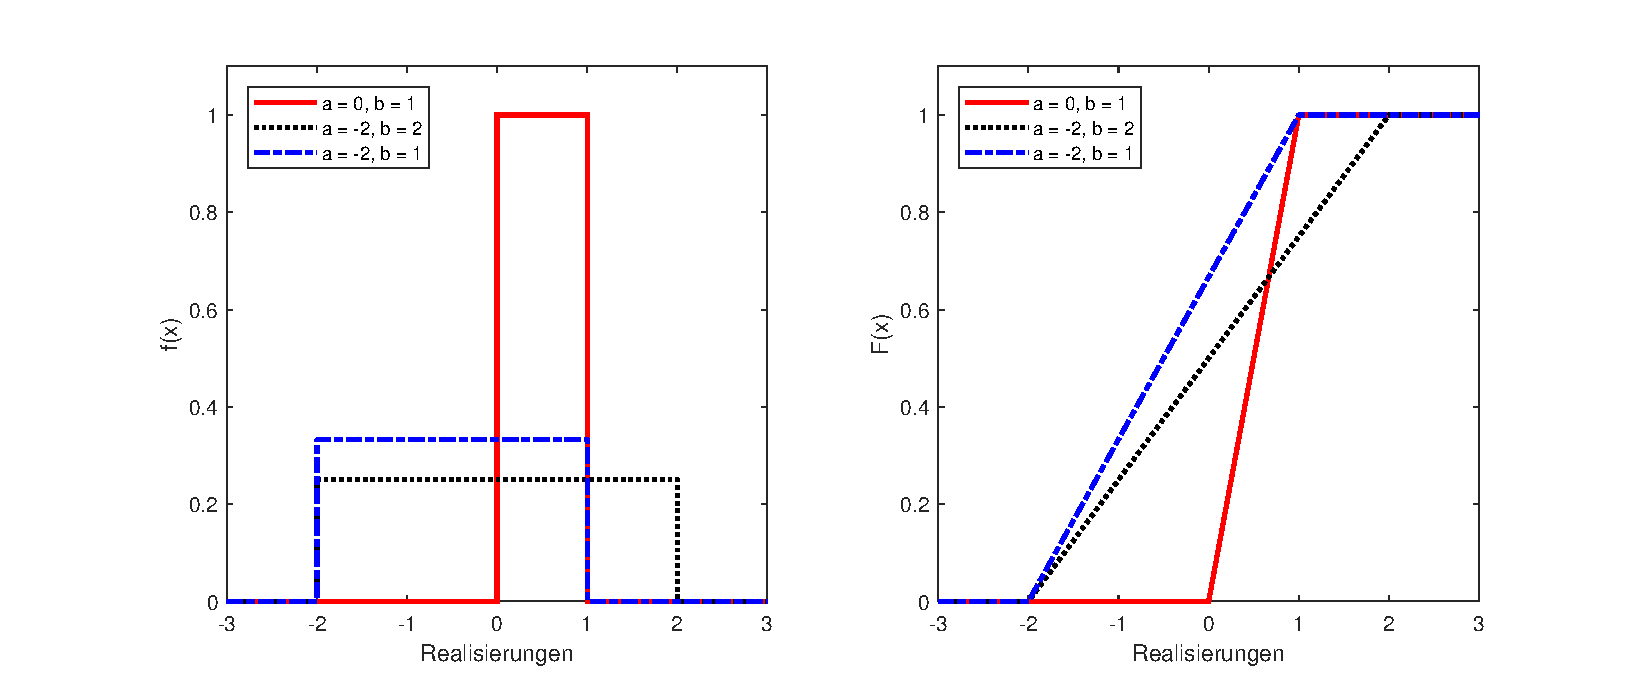
\includegraphics[scale=0.5]{images/plot_con_uniform.eps}
\caption{Dichten (links) und Verteilungsfunktionen (rechts) der stetigen Gleichverteilung mit versch. Parametern}
\end{figure}
\end{frame}

%\begin{frame}
%\frametitle{Die Normalverteilung}
%\begin{block}{Normalverteilung}
%Eine Zufallsvariable $X$ heißt \textit{normalverteilt} mit $\mu$ und $\sigma^2$ wenn
%\[
%f_X(x) = \frac{1}{\sqrt{2\pi\sigma^2}}e^{-\frac{(\mu-x)^2}{2\sigma^2}}
%\]
%gilt. Dies wird kurz durch $X\sim\mathcal{N}(\mu,\sigma^2)$ notiert. 
%\end{block}
%Es gilt:
%\begin{itemize}[<+->]
%\item $\mathbb{E}(X) = \mu$ und Var$(X) = \sigma^2$
%\item $X\sim\mathcal{N}(\mu,\sigma^2) \Rightarrow (a\cdot X-b)\sim\mathcal{N}(a\cdot\mu -b,a^2\sigma^2)$
%\item Das Integral $F(x) = \int f(x) dx$ besitzt für die Normalverteilung keine analytische Form
%\item Die Werte der Verteilungsfunktion $F$ werden numerisch berechnet
%\end{itemize}
%\end{frame}

\begin{frame}
\frametitle{Dichte und Verteilungsfunktion der Normalverteilung}
\begin{figure}[hbtp]
\centering
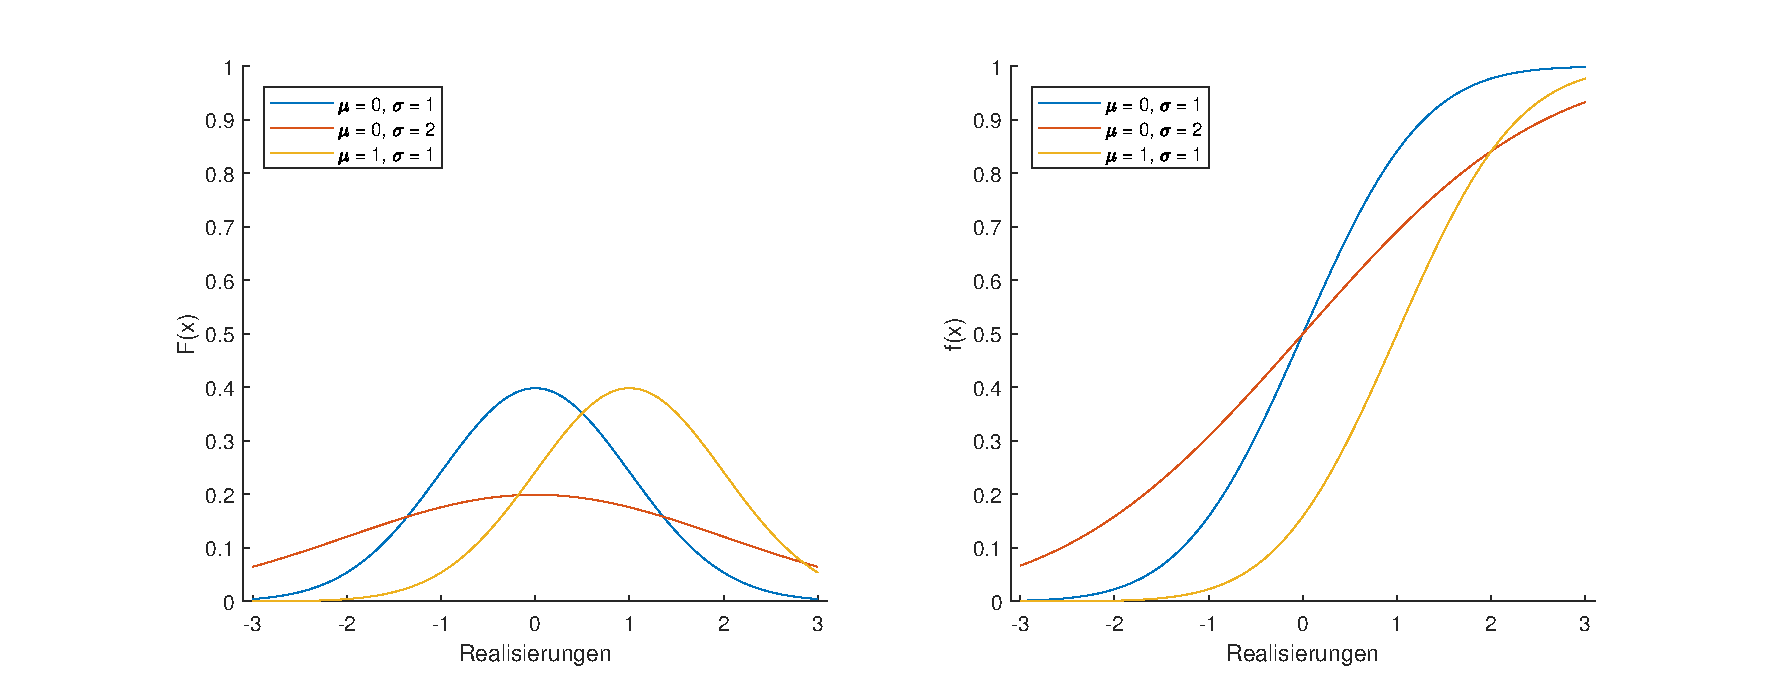
\includegraphics[scale=0.5]{images/plot_normal_dist.eps}
\caption{Dichte (links) und Verteilungsfunktion (rechts) der Normalverteilung bei versch. Parametern}
\end{figure}
\end{frame}

%\begin{frame}
%\frametitle{Das Stab- Balken oder Säulendiagramm}
%\begin{itemize}[<+->]
%\item Einfach Darstellung für die Häufigkeiten verschiedener Kategorien
%\item Seien Merkmale $a_1,\ldots,a_n$ mit absoluten Häufigkeiten $H_{a_1},\ldots,H_{a_n}$ und relativen Häufigkeiten $h_{a_1},\ldots,h_{a_n}$ gegeben
%\item Stabdiagramm: Trage für jedes Merkmal $a$ einen zur x-Achse senkrechten Strich (Stab) mit der Höhe $H_a$ (oder $h_a$) auf
%\item Säulendiagramm: Wie das Stabdiagramm, nur dass hier Säulen statt Striche verwendet werden
%\item Balkendiagramm: Wie das Säulendiagramm, allerdings sind hier die Balken senkrecht zur y-Achse
%\item Bei einem Säulen- oder Balkendiagramm besitzt die Breite der Balken keine Information, d.h. die Breite ist grundsätzlich beliebig
%\end{itemize}
%\end{frame}
%\begin{frame}
%\frametitle{Beispiele für Stab- Balken oder Säulendiagramme}
%\begin{figure}[hbtp]
%\centering
%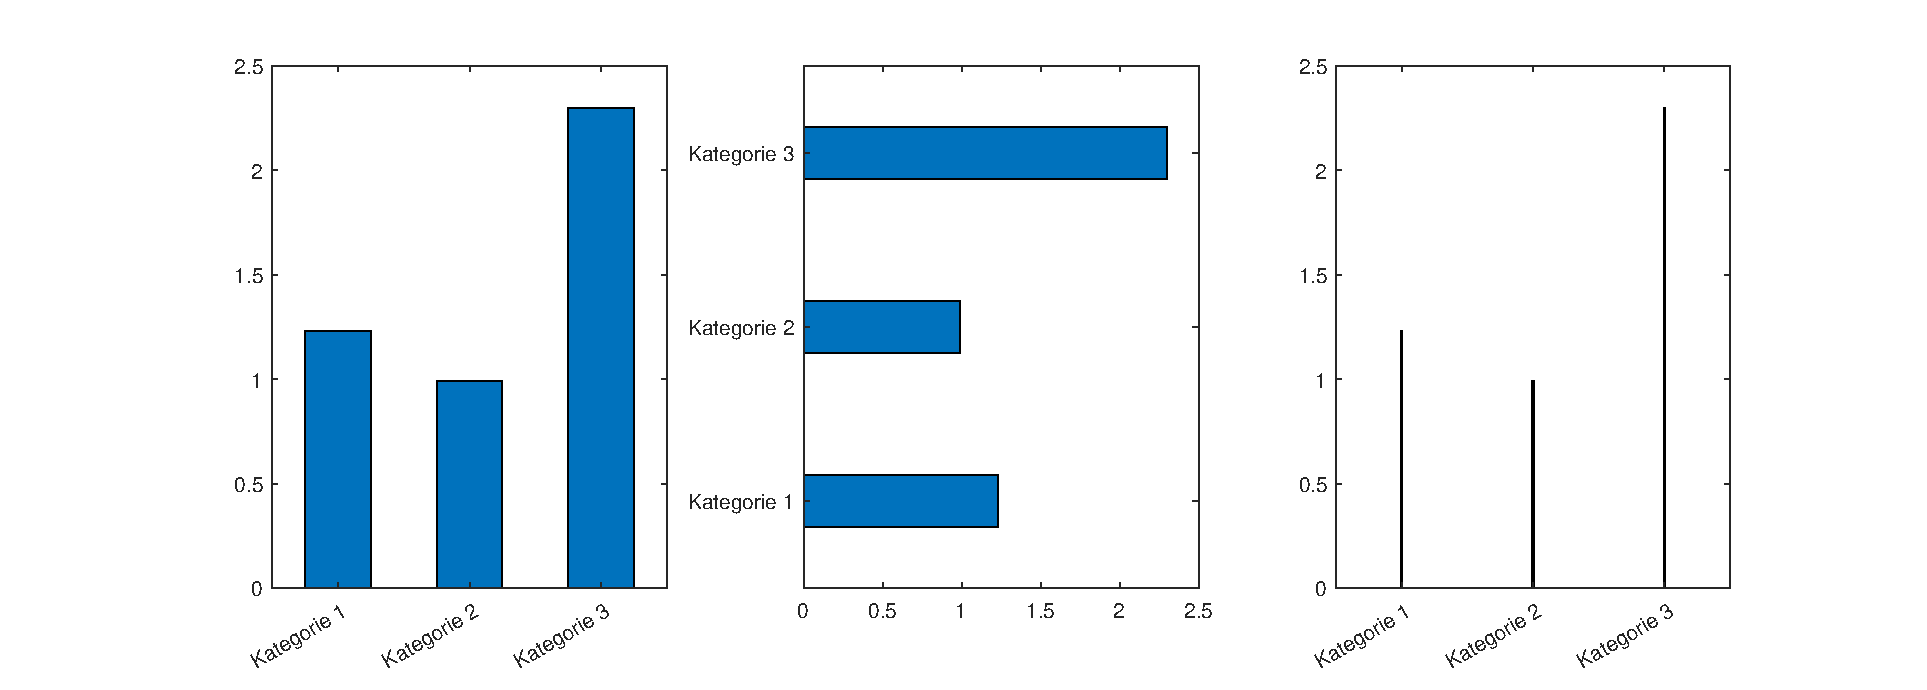
\includegraphics[scale=0.5]{images/barplot.eps}
%\caption{Beispiel für ein Säulendiagramm (links), Balkendiagramm (mittig) und Balkendiagramm (rechts)}
%\end{figure}
%\end{frame}
%\begin{frame}
%\frametitle{Das Histogramm}
%\begin{itemize}[<+->]
%\item Bei den Balken- und Säulendiagrammen hatte die jeweilige Breite keine Bedeutung
%\item Ein der Verdopplung der Breite eines Balken würde jedoch optisch diesem Balken eine höhere Bedeutung zuweisen
%\item Wir betrachten nun viele Ausprägungen mit zumindest metrisch-skalierten Merkmalen
%\item Gegeben seien zunächst Gruppierungen der Merkmale in Intervalle der Form $[c_0,c_1),[c_1,c_2),\ldots,[c_{k-1},c_k)$
%\item Sei $h_j$ hier die relative Häufigkeit der Beobachtung im Intervall $[c_{j-1},c_j)$ und $H_j$ entsprechend die absolute Häufigkeit
%\item Über diesen Intervallen werden nun Rechtecke mit der Breite $d_j=c_j-c_{j-1}$ und Höhe $\frac{h_j}{d_j}$ (bzw. $\frac{H_j}{d_j}$) gezeichnet
%\item Die Summe der Flächen aller Rechtecke ist gleich $1$ (bzw. gleich $n$)
%\item Die Klassenbreiten sollten wenn möglich sinnvoll und annähernd gleich sein
%\item Neben der subjektiven optischen Begutachtung, existieren verschiedene Faustregeln für die Anzahl der Klassen, wie z.B.
%\[
%k = \lfloor\sqrt{n}\rfloor ,\quad k = 2\lfloor\sqrt{n}\rfloor  \quad\text{oder}\quad k = \lfloor 10 \log_{10} n \rfloor
%\]
%\end{itemize}
%\end{frame}
%\begin{frame}
%\frametitle{Beispiel für ein Histogramm}
%\begin{figure}[hbtp]
%\centering
%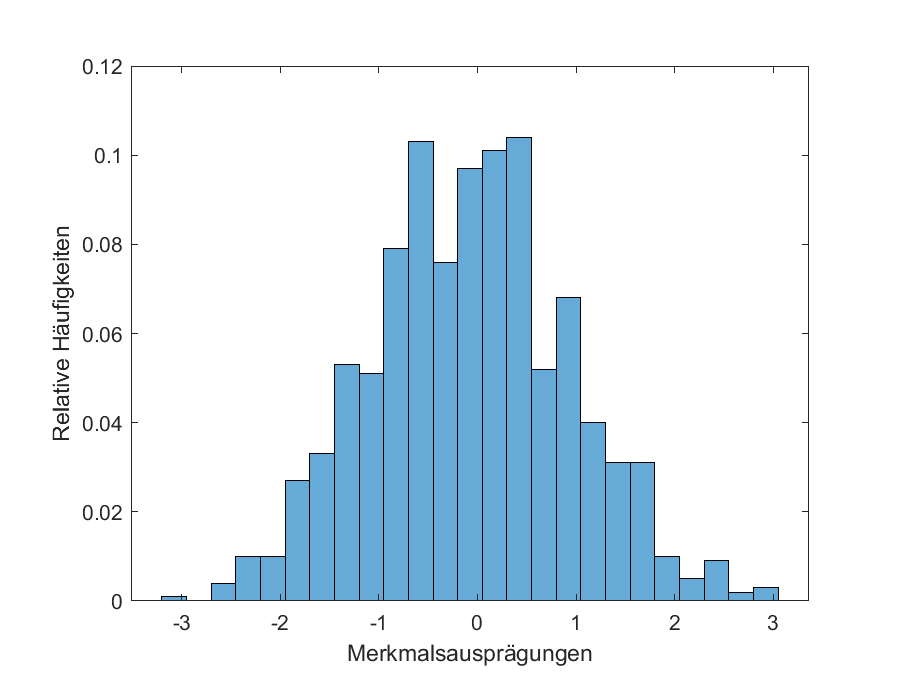
\includegraphics[scale=0.55]{images/plot_histogram.eps}
%\caption{Histogramm für 1000 Pseudozufallszahlen über 25 äquidistante Klassen}
%\end{figure}
%\end{frame}
%\begin{frame}
%\frametitle{Das Streudiagramm}
%Für zwei stetige Merkmale $X$ und $Y$ mit paarweisen Ausprägungen $(x_1,y_1),(x_2,y_2),\ldots,(x_n,y_n)$ kann das sogenannte Streudiagramm als einfache Visualisierung verwendet werden:
%\begin{block}{Streudiagramm}
%Die  Darstellung  der  Messwertepaare $(x_1,y_1),(x_2,y_2),\ldots,(x_n,y_n)$ im (x,y)-Koordinatensystem heißt \textit{Streudiagramm} (engl. scatter plot).
%\end{block}
%\end{frame}
%\begin{frame}
%\frametitle{Beispiel für ein Streudiagramm}
%\begin{figure}[hbtp]
%\centering
%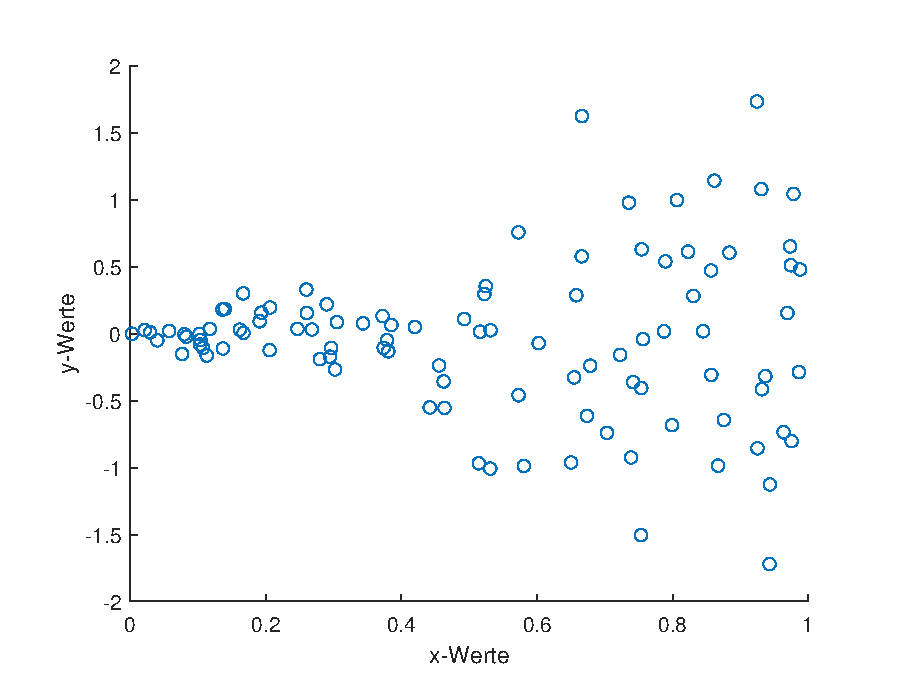
\includegraphics[scale=0.55]{images/plot_scatter.eps}
%\caption{Beispiel für ein Streudiagramm mit 100 Wertepaaren}
%\end{figure}
%\end{frame}
%\begin{frame}
%\frametitle{Der Box-Plot}
%In einem Box-Plot wird die 5-Punkte-Zusammenfassung ($x_{min},x_{0.25},x_{med},x_{0.75},x_{max})$ grafisch aufbereitet.
%\begin{enumerate}
%\item Anfang der Box bei $x_{0.25}$ mit beliebiger Höhe\\
%Ende der Box bei $x_{0.75}$ (damit ist die Länge der Box gleich dem Interquartilsabstand)
%\item Die Box wird auf Höhe des Medians mit einem vertikalen Strich geteilt
%\item Von den Rändern der Box werden horizontale Linien bis $x_{min}$ bzw. $x_{max}$ gezogen, die mit einer vertikalen Linie abgeschlossen werden
%\end{enumerate}
%Oft wird ein Box-Plot vertikal aufgebaut, so sind Minimum und Maximum unten bzw. oben, statt links und rechts.
%\end{frame}
%\begin{frame}
%\frametitle{Beispiel für einen Box-Plot}
%\begin{figure}[hbtp]
%\centering
%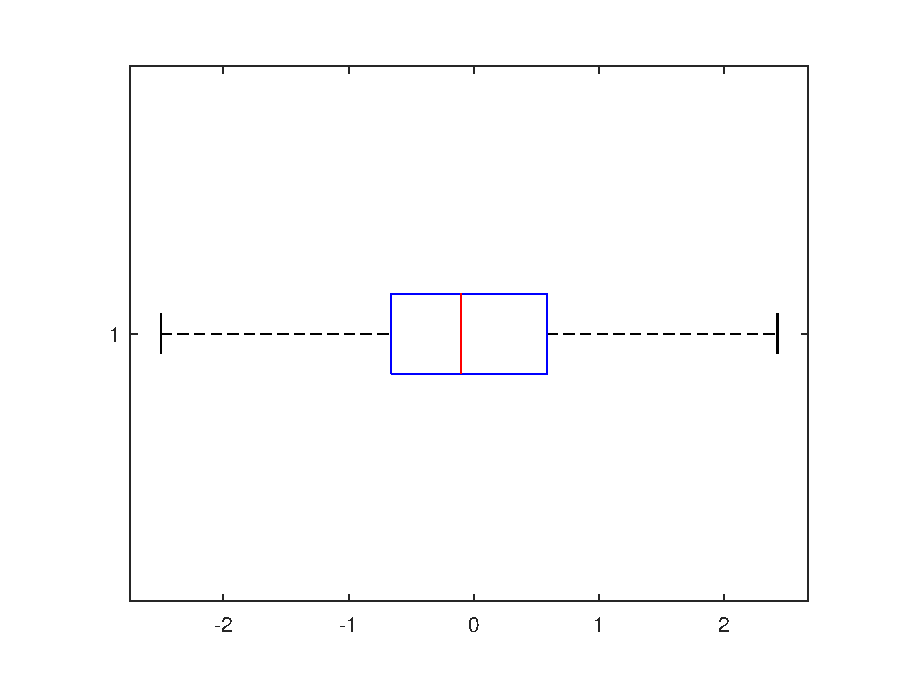
\includegraphics[scale=0.55]{images/plot_boxplot.eps}
%\caption{Beispiel für einen Boxplot}
%\end{figure}
%\end{frame}
%\begin{frame}
%\frametitle{Die Heatmap}
%\begin{itemize}[<+->]
%\item Wir betrachten Daten, die in einer Matrix $M$ dargestellt werden
%\item Der Eintrag $M_{(i,j)}$ hängt von dem $i$-ten Zeilenmerkmal und dem $j$-ten Spaltenmerkmal ab
%\item Die Zeilenmerkmale und Spaltenmerkmale können die gleichen oder verschiedene Merkmale sein
%\item Der numerische Wert $M_{(i,j)}$ wird im Vergleich zu den übrigen Werten von $M$ farblich kodiert
%\item Die Kategorien werden an den Zeilen und Spalten aufgetragen und jede Zelle entsprechend ihrer Farbe eingefärbt
%\item Die Farbskala wird als Legende mit angegeben
%\item Optional können die Zellenwerte mit in die Heatmap aufgenommen werden
%\end{itemize}
%\end{frame}
%\begin{frame}
%\frametitle{Beispiel I für eine Heatmap}
%\begin{figure}[hbtp]
%\centering
%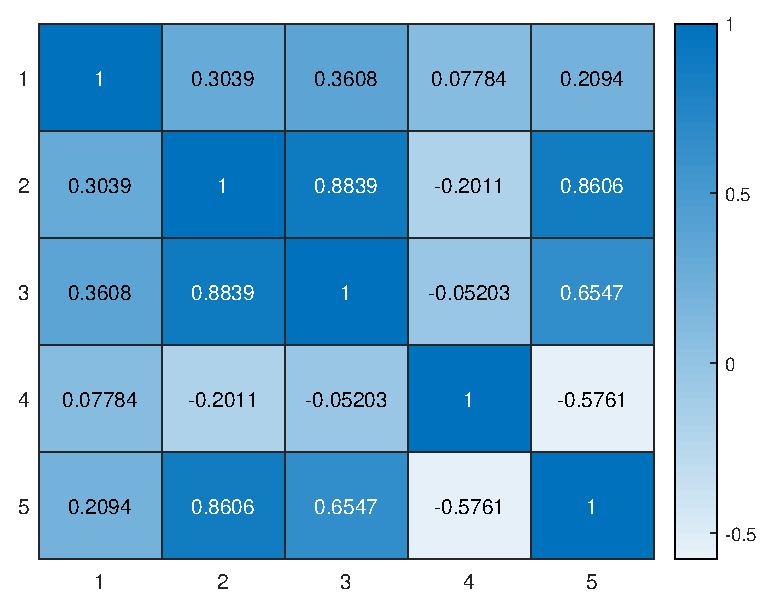
\includegraphics[scale=0.55]{images/plot_heatmap_corr.eps}
%\caption{Beispiel für eine Heatmap einer Korrelationskoeffizientenmatrix}
%\end{figure}
%\end{frame}
%\begin{frame}
%\frametitle{Beispiel II für eine Heatmap}
%\begin{figure}[hbtp]
%\centering
%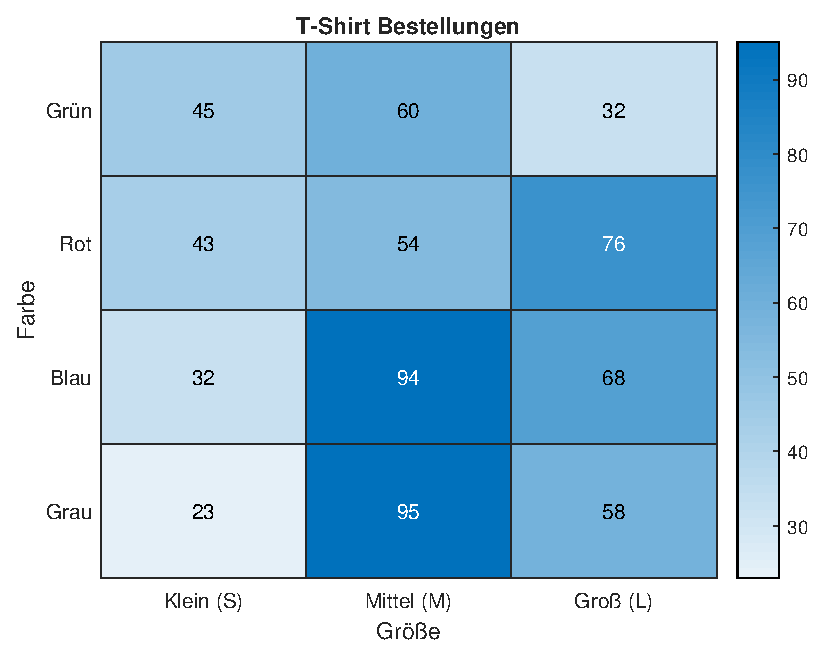
\includegraphics[scale=0.55]{images/plot_heatmap_tshirt.eps}
%\caption{Beispiel für eine Heatmap zu T-Shirt Verkäufen}
%\end{figure}
%
%\end{frame}
%\begin{frame}
%\frametitle{Regeln für gute Diagramme}
%\begin{enumerate}[<+->]
%\item Diagramme sollen Informationen übersichtlich darstellen, d.h. sie sollten erst bei einer hinreichend großen Anzahl von Informationen, die vermittelt werden sollen, eingesetzt werden
%\item Diagramme sollen selbsterklärend und übersichtlich sein
%\item Die Beschriftung eines Diagrammes ist vollständig, dazu gehören unter Berücksichtigung der Übersichtlichkeit (und sofern anwendbar)
%\begin{itemize}[<+->]
%\item Titel
%\item Zeitraum
%\item Ortsangabe
%\item Achsenbeschriftungen
%\item Angabe einer Legende
%\item Quelle
%\end{itemize}
%\item 3D-Darstellungen nur dann, wenn das Volumen eine sinnvolle Bedeutung hat (Nicht aus optischen Gründen)
%\item Sprünge in Achse müssen deutlich gekennzeichnet werden
%\item Die Darstellung sollte proportional sein, insbesondere betrifft dies Höhe, Breite und Abstände
%\end{enumerate}
%\end{frame}